\documentclass[12pt,letterpaper]{article}

\usepackage[utf8]{inputenc}
\usepackage[T1]{fontenc}
\usepackage[english]{babel}
\usepackage{listings, float}
\usepackage{graphicx, geometry, xcolor, amsmath, enumitem}
\usepackage[normalem]{ulem}
\usepackage[colorlinks=true, linkcolor=linkblue, urlcolor=linkblue, citecolor=linkblue]{hyperref}

\geometry{margin=3cm, top=3cm, bottom=3cm}

\renewcommand{\lstlistingname}{Código}

%------ Definimos los colores para la sintaxis del código --------%
\definecolor{backcolour}{rgb}{0.93, 0.93, 0.93} % Gris suave para el fondo
\definecolor{codegreen}{rgb}{0, 0.6, 0}         % Comentarios
\definecolor{codegray}{rgb}{0.5, 0.5, 0.5}      % Números de línea
\definecolor{codepurple}{rgb}{0.58, 0, 0.82}    % Strings
\definecolor{keywordcolor}{rgb}{0.5, 0.0, 0.5}
\definecolor{codeorg}{HTML}{DB9400}      % Tipos de datos y Structs propios

% --- Configuración del Estilo ---
\lstdefinestyle{modernc}{
    language=C,
    backgroundcolor=\color{backcolour},   
    commentstyle=\color{codegreen},
    keywordstyle=\color{keywordcolor}\bfseries,
    numberstyle=\tiny\color{codegray},
    stringstyle=\color{codepurple},
    basicstyle=\ttfamily\footnotesize,
    breakatwhitespace=false,
    breaklines=true,
    captionpos=b,
    keepspaces=true,
    numbers=left,
    numbersep=5pt,
    showspaces=false,                
    showstringspaces=false,
    showtabs=false,                  
    tabsize=4,
    frame=single,
    rulecolor=\color{black!20},
    frameround=tttt,
    emph={int,uint32_t,char,double,float,unsigned,void,bool,struct,size_t,
          Room, Client, pthread_mutex_t, NULL},
    emphstyle=\color{codeorg}\bfseries
}

% --- Estilo Assembly ---
\lstdefinestyle{modernasm}{
    language=Assembler,
    backgroundcolor=\color{backcolour},
    commentstyle=\color{codegreen},
    keywordstyle=\color{keywordcolor}\bfseries,
    numberstyle=\tiny\color{codegray},
    stringstyle=\color{codepurple},
    basicstyle=\ttfamily\footnotesize,
    breaklines=true,
    captionpos=b,
    numbers=left,
    numbersep=5pt,
    frame=single,
    rulecolor=\color{black!20},
    frameround=tttt,
    morecomment=[l]{;},
    morekeywords={
        mov, add, sub, mul, div, inc, dec,
        push, pop, call, ret,
        cmp, jmp, je, jne, jg, jl, jge, jle,
        and, or, xor, not,
        lea, nop
    },
    emph={
        eax, ebx, ecx, edx,
        esi, edi, esp, ebp,
        ax, bx, cx, dx,
        rax, rbx, rcx, rdx,
        rsi, rdi, rsp, rbp
    },
    emphstyle=\color{codeorg}\bfseries
}

\definecolor{linkblue}{HTML}{1A167A}

\begin{document}

\begin{titlepage}
  \thispagestyle{empty}
  %--------------- COMANDO LINEA----------------->
  \newcommand{\linea}{\rule{\linewidth}{0.5mm}}                 
  \center
  %<<<<<<<<<<<<<<<<<<<<<<<<<<<<<<<<<<<<<<<<<<<

  %Add logos
  \includegraphics[width=0.24\textwidth]{~/unam_logo.png} \hspace{1.5cm}
  \includegraphics[width=0.25\textwidth]{~/fc_logo.png} \\[1cm]
  \textbf{\Large UNIVERSIDAD NACIONAL AUTÓNOMA}\\[3mm]
  \textbf{\Large DE MÉXICO} \\[6mm]
  \textit{\Large Facultad de Ciencias}

  \vfill

  %---------------TÍTULO----------------->
  \linea
  \vfill \vspace{1cm}
  \textbf{\Large Sistemas Operativos}\\[1.1cm]
  \textbf{\Large Sincronización de Tareas\\ y Gestión de Recursos (Semáforos)}\\[0.9cm]
  \linea \\
  \vfill
  \vspace{0.7cm}
  %Title of the Research
  \textbf{\Large  Práctica 5}\\[6mm]
  %<<<<<<<<<<<<<<<<<<<<<<<<<<<<<<<<<<<<<<<<<<<

  %Team
  \vfill
  \textit{\small Presenta:}\\
  \textbf{\large \textbf{Rojo Peña Manuel Ianluck}}\\[3mm]

  %Profesor y Grupo
  \textit{\small Profesor:}\\
  \textbf{Javier León Cotonieto}\\[3mm]
  \textit{\small Ayudante laboratorio:}\\
  \textbf{Adrián Martínez Manzo}\\[3mm]
  \small Grupo: 7004, 2026-2\\[3mm]
  \vfill

  %Fecha or Date
  \textit{\small Fecha de entrega:}\\
         {\large 30 de marzo, 2026}
         
\end{titlepage}


\newpage

\section*{Introducción}

Los sistemas operativos modernos con planificación expropiativa permiten que múltiples tareas compartan el procesador de forma transparente, sin embargo, esta capacidad introduce un problema fundamental: cuando dos o más tareas acceden concurrentemente a un recurso compartido sin coordinación, el sistema puede producir resultados incorrectos o incluso colapsar.\\

\noindent
En esta práctica implementaremos, desde el nivel del \textit{kernel}, un conjunto de primitivas de sincronización basadas en semáforos para resolver dicho problema sobre el planificador \textit{Round Robin} realizado en la práctica anterior.

\subsection*{Planteamiento del problema}

Simularemos el firmware de un satélite tipo \textit{CubeSat} con cinco subsistemas concurrentes, cada subsistema debe realizar dos operaciones en su ciclo: encender un calentador térmico (un \texttt{LED} en este caso) durante 500\,ms y, una vez ``caliente'', transmitir un reporte de telemetría por el único canal de radio disponible (print por el puerto \texttt{UART}/\texttt{USB}). Este sistema impone dos restricciones físicas críticas:

\begin{itemize}
\item \textbf{Límite de energía:} la fuente de alimentación solo soporta un máximo de tres calentadores (LEDs) encendidos simultáneamente. Superar ese límite provoca un \textit{brownout} eléctrico y la pérdida del satélite.
\item \textbf{Exclusividad del radio:} el canal \texttt{UART} es un recurso único, si dos tareas escriben al mismo tiempo, el mensaje recibido en tierra es ilegible.
\end{itemize}

El objetivo central de la práctica es, primero, observar las fallas que surgen de forma natural cuando se ignoran estas restricciones (\textbf{Fase A}), y después resolverlas mediante la implementación de semáforos a nivel kernel (\textbf{Fase B}).

\newpage

\section*{Conceptos Clave}

\subsubsection*{Condición de carrera (\textit{Race Condition}).}
Situación que ocurre cuando dos o más tareas acceden y modifican un recurso compartido de forma concurrente y el resultado final depende del orden de ejecución. En un planificador expropiativo, el \textit{quantum} puede expirar en cualquier instrucción, por lo que ninguna secuencia de instrucciones que involucre un recurso compartido es segura por defecto.

\subsubsection*{Sección crítica.}
Fragmento de código que accede a un recurso compartido y que no debe ser ejecutado por más de una tarea a la vez. Protegerla correctamente es el objetivo de los mecanismos de sincronización.

\subsubsection*{Semáforo.}
Primitiva de sincronización propuesta por Dijkstra. Consiste en un contador entero y dos operaciones atómicas:
\begin{itemize}
\item \texttt{wait} (P / \texttt{sem\_wait}): si el contador es mayor que cero, lo decrementa y la tarea continúa; si es cero, la tarea se bloquea hasta que el recurso se libere.
\item \texttt{post} (V / \texttt{sem\_post}): incrementa el contador o desbloquea a la primera tarea en espera.
\end{itemize}

\subsubsection*{Mutex (semáforo binario).}
Semáforo inicializado en 1 que garantiza acceso exclusivo a un recurso, solo una tarea puede estar dentro de la sección crítica en un instante dado.

\subsubsection*{Semáforo contador.}
Semáforo inicializado en $N > 1$ que permite hasta $N$ tareas simultáneas. Para esta práctica lo usamos con $N = 3$ para limitar los calentadores activos.

\subsubsection*{Estado BLOCKED.}
Estado adicional del Bloque de Control de Tarea (TCB) en el que la tarea cede el CPU voluntariamente sin consumir su \textit{quantum}. El planificador ignora por completo las tareas en este estado, eliminando el desperdicio de ciclos del \textit{busy-waiting}.

\newpage

\section*{Fase A: El Caos de la Concurrencia\\ (Implementación Ingenua)}

\subsection*{Objetivo y procedimiento}

El propósito de esta fase es exponer, de forma deliberada, las fallas que produce un planificador \textit{Round Robin} puro cuando múltiples tareas comparten recursos sin ningún mecanismo de protección. Para ello, implementamos cinco tareas (\texttt{task\_subsystem1} a \texttt{task\_subsystem5}), cada una asociada a un LED distinto, que ejecutan indefinidamente el siguiente ciclo:

\begin{enumerate}
\item Encender el LED correspondiente (calentador ON).
\item Esperar 500\,ms mediante \texttt{delay\_cycles\_exact()} (simulación del calentamiento térmico).
\item Apagar el LED (calentador OFF).
\item Imprimir por UART un mensaje largo de telemetría mediante \texttt{printf}.
\end{enumerate}

\noindent
El respectivo código que se implementó para ello está en \texttt{user\_app.c} y es el siguiente:

\begin{lstlisting}[style=modernc]
#include <stdint.h>
#include <stdio.h>
#include "syscalls.h"

#define LED_0 5
#define LED_1 8
#define LED_2 10
#define LED_3 13
#define LED_4 15
#define DELAY_500MS 20850000

void
task_subsystem1(void)
{
  sys_gpio_dir(LED_0, 1);

  while (1) {
    sys_gpio_set(LED_0, 1);
    delay_cycles_exact(DELAY_500MS);
    sys_gpio_set(LED_0, 0);
    printf("[1st SUBSYSTEM]: Calentamiento finalizado. Operacion nominal alcanzada. Transfiriendo paquetes de telemetria y reportando estado actual a base terrestre...\n");
  }
}
\end{lstlisting}

\bigskip

\noindent
La misma función la utilizamos para \texttt{task\_subsystem2}, \texttt{task\_subsystem3}, \texttt{task\_subsystem4} y \texttt{task\_subsystem5} pero prendiendo y apagando un LED distinto.\\

\noindent
Las cinco tareas se encolaron simultáneamente al inicio del sistema, sin semáforos ni región crítica de ningún tipo con \textit{quantum} del \textit{SysTick} en 10\,ms.

\subsection*{Caso 1. Mensaje estándar}
En el primer experimento se utilizó el mensaje de telemetría tal como lo especifica la práctica. Contrario a lo esperado, la terminal no mostró corrupción visible, los mensajes de los cinco subsistemas se imprimían de forma aparentemente ordenada y los LED's permanecían encendidos de manera estable (con más de 5 prendidos en caso de encolar 5 tareas), con algún parpadeo ocasional.\\

La ausencia del fallo se explica por la arquitectura interna de la comunicación serie en el RP2040, la función \texttt{printf} del \textit{pico-sdk} no escribe directamente al hardware UART byte a byte; en cambio, deposita los datos en un \textbf{buffer circular de software} gestionado por la pila USB-CDC (TinyUSB). La escritura en ese buffer es suficientemente rápida para completarse dentro de un único \textit{quantum} de 10\,ms cuando el mensaje es corto, de modo que el planificador casi nunca interrumpe la transmisión a mitad del texto.\\

Adicionalmente, el flujo de control USB introduce retardos de sincronización entre paquetes que, de forma fortuita, separan temporalmente las escrituras de distintas tareas. En consecuencia, aunque no existe ninguna protección explícita, la granularidad del mensaje y los tiempos de la pila USB impiden que la condición de carrera se manifieste de forma perceptible.\\

\noindent
Podemos ver las evidencia de este caso en el siguiente video:\\

\href{https://drive.google.com/file/d/1uVFFZONrw-ooMVKhCwuL4oLu651Wa1V4/view?usp=drive_link}
     {\textbf{\textit{\textcolor{linkblue}{Evidencia Práctica 5. Fase A: Caso 1}}}}

\subsection*{Caso 2. Intento de forzar el fallo (colapso de la terminal)}
Para intentar reproducir la corrupción esperada se incrementó la longitud del mensaje de telemetría y se redujo el intervalo entre impresiones, con el objetivo de que varias tareas escribieran en el buffer USB de forma solapada.\\

\begin{lstlisting}[style=modernc]
void
task_subsystem1(void)
{
  sys_gpio_dir(LED_0, 1);

  while (1) {
    sys_gpio_set(LED_0, 1);
    delay_cycles_exact(DELAY_500MS);
    sys_gpio_set(LED_0, 0);
    printf("[1st SUBSYSTEM]: Calentamiento finalizado. Operacion nominal alcanzada. Transfiriendo paquetes de telemetria y reportando estado actual a base terrestre...\n Lorem ipsum dolor sit amet consectetur adipiscing elit suscipit metus, sagittis phasellus porta convallis luctus maecenas dui quam quis sem, accumsan placerat odio pharetra feugiat ac platea cursus. Duis aptent elementum tortor curae maecenas dui hac ridiculus vivamus sociosqu himenaeos semper, sociis mi viverra proin eget venenatis malesuada velit egestas eleifend nascetur. Ridiculus a tincidunt odio leo fermentum taciti varius velit dui ultricies ultrices, morbi lacus conubia molestie fusce torquent integer convallis ligula.\n \nQuisque nunc habitasse fames himenaeos nascetur placerat praesent, maecenas a sociis semper curae ornare. Pharetra odio senectus libero magna purus vel sociosqu himenaeos suscipit, mauris condimentum velit cras habitant curae integer in dictumst arcu, ut interdum vitae tempor auctor vestibulum ultrices donec. Egestas duis inceptos sociosqu nec vestibulum aliquam quam magnis dui, hac quisque ultrices metus vel pharetra euismod velit eros, curabitur a turpis quis ante iaculis fames litora.\n");
  }
}
\end{lstlisting}

\bigskip
  
\noindent
No obstante, el resultado fue que la terminal dejó de responder, dejó de mostrar nuevos caracteres y no procesó ninguna entrada del teclado, por lo que se tuvo que forzar el cierre de la terminal, además de que siguen más de 3 LED's activos. Este comportamiento se debe a que, al saturar el buffer de transmisión USB-CDC más rápido de lo que el \textit{host} puede drenarlo, la pila TinyUSB alcanza su límite de capacidad y descarta silenciosamente los datos entrantes o congela la transmisión.\\
  
Desde el punto de vista del \textit{host}, el flujo de caracteres se detiene de forma abrupta, la terminal no recibe más bytes y permanece bloqueado esperando datos que nunca llegan, aparentando estar ``roto''. La falla, en este caso, se produce en la capa de transporte serie antes de que la condición de carrera a nivel de instrucciones pueda siquiera manifestarse en pantalla. Incluso, en algunas situaciones, basta con avticar dos tareas para romper la terminal, dejando solo los LED's de dichas tareas activos.\\

\noindent
Podemos ver de nuevo, las evidencia a este \textbf{caso 2} en el siguiente video:\\

\href{https://drive.google.com/file/d/1uVFFZONrw-ooMVKhCwuL4oLu651Wa1V4/view?usp=sharing&t=74}
     {\textbf{\textit{\textcolor{linkblue}{Evidencia Práctica 5. Fase A: Caso 2}}}}

\newpage

\section*{Fase B: El Orden del SO\\ (Implementación de Semáforos)}
En esta fase se modificó el kernel para soportar sincronización real mediante semáforos, eliminando las condiciones de carrera identificadas en la \textbf{Fase A}. Los cambios se hicieron en tres archivos: \texttt{scheduler.h}, \texttt{scheduler.c} y \texttt{user\_app.c}.

\subsection*{Modificaciones al Kernel}

\subsubsection*{\texttt{scheduler.h}: Nuevas estructuras de datos}
Se agregó al header el estado \texttt{BLOCKED} en \texttt{task\_state\_t} y la estructura \texttt{semaphore\_t}, junto con los prototipos de las tres funciones de semáforo.

\begin{lstlisting}[style=modernc, caption={\texttt{scheduler.h}, Estado \texttt{BLOCKED} y estructura \texttt{semaphore\_t}}]
#ifndef SCHEDULER_H
#define SCHEDULER_H

#include <stdint.h>

#define MAX_TASKS 5
#define STACK_SIZE 256 // 256 palabras de 32 bits = 1KB por tarea

// Estados posibles de una tarea
typedef enum {
  DORMANT, // Inactiva, no esta en la cola
  READY,   // Lista para ejecutarse
  RUNNING, // Ejecutandose actualmente
  BLOCKED  // Esperando mutex
} task_state_t;

// Task Control Block
typedef struct {
  uint32_t *sp;                  // Puntero de Pila actual
  task_state_t state;            // Estado de la tarea
  uint32_t stack[STACK_SIZE];    // Espacio de memoria de la pila
  void (*entry_point)(void);     // Funcion de la tarea
  uint8_t quantum;   //priority quantum
  uint8_t remaining; //quantum countdown
} tcb_t;

// Semaphore (mutex and counter)
typedef struct {
  int count;            // Available resources (count >= 0)
  int queue[MAX_TASKS]; // FIFO queue of blocked task IDs
  int head;             // Read index
  int tail;             // Write index
  int size;             // Number of currently blocked tasks
} semaphore_t;
 
//Semaphore prototypes
void semaphore_init (semaphore_t *sem, int initial_count);
void sys_semaphore_wait(semaphore_t *sem);
void sys_semaphore_post(semaphore_t *sem);

#endif
\end{lstlisting}

\subsubsection*{\texttt{scheduler.c}: Implementación de los semáforos}
Se implementaron las tres funciones de semáforo, el punto importante desarrollado es que, \texttt{sys\_semaphore\_wait} \textbf{no realiza busy-waiting}, sino que, cuando el recurso no está disponible, cambia el estado de la tarea a \texttt{BLOCKED} y dispara \texttt{PendSV} de inmediato, cediendo el CPU genuinamente.\\

Además, se actualizó \texttt{schedule()} para que preserve el \textit{stack pointer} (\texttt{sp}) de las tareas bloqueadas sin cambiarlas a \texttt{READY}.

\begin{lstlisting}[style=modernc, caption={\texttt{scheduler.c}, \texttt{semaphore\_init}, \texttt{sys\_semaphore\_wait} y \texttt{sys\_semaphore\_post}}]
/**
 * Semaphores
 **/

/**
 * @brief Initialize a semaphore with the given resource count.
 */
void
semaphore_init(semaphore_t *sem,
               int initial_count)
{
  sem->count = initial_count;
  sem->head  = 0;
  sem->tail  = 0;
  sem->size  = 0;
  for (int i = 0; i < MAX_TASKS; i++)
      sem->queue[i] = -1;
}

/**
 * @brief Request for resource to the semaphore.
 * - If resources are available (count > 0), then decrement it and continue.
 * - If not (count == 0):
 *  + BLOCKED current task.
 *  + We queue it con the semaphore waiting queue
 *  + Force PendSV so the scheduler selects another task.
 *
 *  No busy-waiting implemented, the task yields CPU genuily.
 */
void
sys_semaphore_wait(semaphore_t *sem)
{
  //Critical section: disable interrupts atomically
  uint32_t primask;
  __asm volatile ("MRS %0, PRIMASK" : "=r"(primask));
  __asm volatile ("CPSID i"); //defuse IRQs
  
  if (sem->count > 0) {
    //Resource available, we take it and continue without BLOCKING
    sem->count--;
    __asm volatile ("CPSIE i"); //refuse IRQs
    return;
  }

  //No resources, BLOCK current task
  tasks[current_task].state = BLOCKED;

  //Enqueue the task ID in the semaphore's circular FIFO
  sem->queue[sem->tail] = current_task;
  sem->tail = (sem->tail + 1) % MAX_TASKS;
  sem->size++;

  __asm volatile ("CPSIE i"); //Re-enable interrupts before triggering PendSV

  //Yield the CPU to scheduler
  //The resource is considered acquired at that point (count unchanged).
  trigger_pendsv();
}

/**
 * @brief Release one resource back to the semaphore.
 *
 * - If tasks are waiting:
 *     wake the first one (FIFO) and transfer the resource directly (count stays the same).
 * - If nobody is waiting:
 *     increment count.
 */
void
sys_semaphore_post(semaphore_t *sem)
{
  //Disable interrupts atomically
  uint32_t primask;
  __asm volatile ("MRS %0, PRIMASK" : "=r"(primask));
  __asm volatile ("CPSID i");

  if (sem->size > 0) {
    //Wake the oldest waiting task
    int woken_id = sem->queue[sem->head];
    sem->queue[sem->head] = -1;
    sem->head = (sem->head + 1) % MAX_TASKS;
    sem->size--;

    //Transfer resource directly, BLOCKED -> READY
    //count is NOT incremented the resource passes directly
    tasks[woken_id].state = READY;

  } else {
    //Nobody waiting, we return the resource to the semaphore
    sem->count++;
  }

  __asm volatile ("CPSIE i");
}
\end{lstlisting}

\bigskip

\noindent
La modificación correspondiente en \texttt{schedule()} garantiza que las tareas bloqueadas conserven su \textit{stack pointer} sin ser reinsertadas en la cola de listos:

\begin{lstlisting}[style=modernc, caption={\texttt{scheduler.c}, \texttt{schedule()} maneja el estado \texttt{BLOCKED}}]
uint32_t
schedule(uint32_t current_sp)
{
  // Save the SP of the task that was just paused
  if (current_task != -1 && tasks[current_task].state == RUNNING) {
    tasks[current_task].sp = (uint32_t *)current_sp;
    tasks[current_task].state = READY; // Put it back in the ready queue
  } else if (current_task != -1 && tasks[current_task].state == BLOCKED) {
    //Keep SP but without changing its state, stays BLOCKED
    tasks[current_task].sp = (uint32_t *)current_sp;
  }

  // Round Robin algorithm
  int next_task = current_task;
  int tries = 0;

  do {
    next_task = (next_task + 1) % MAX_TASKS;
    tries++;
    // If we find a ready task, stop searching
    if (tasks[next_task].state == READY)
      break;
  } while (tries < MAX_TASKS);
  
  // If a runnable task was found
  if (tasks[next_task].state == READY) {
    current_task = next_task;
    tasks[current_task].state = RUNNING;
    //Reaload quantum with the income one
    tasks[current_task].remaining = tasks[current_task].quantum;
    return (uint32_t)tasks[current_task].sp;
  }

  // If no task is ready, keep the current context
  //  return current_sp;
  return 0; 
}
\end{lstlisting}

\bigskip

\subsubsection*{\texttt{user\_app.c}: Tareas con semáforos}
Cada tarea adquiere primero \texttt{sem\_energia} (semáforo contador, init\,=\,3) antes de encender su LED, y lo libera al apagarlo, luego adquiere \texttt{sem\_radio} (mutex, init\,=\,1) antes del \texttt{printf} y lo libera al terminar.\\

Se muestra la tarea 1 como representativa, las demás son idénticas cambiando el pin y el número de subsistema.

\begin{lstlisting}[style=modernc, caption={\texttt{user\_app.c}, semaphores declared and \texttt{task\_subsystem1}}]
// Semaphores defined in main.c
extern semaphore_t sem_radio;   //Mutex(init=1): exclusive UART access
extern semaphore_t sem_energia; //Counter(init=3): max 3 LEDs on at once

void
task_subsystem1(void)
{
  sys_gpio_dir(LED_0, 1);
  while (1) {
      // Thermal heater phase
      sys_semaphore_wait(&sem_energia); //acquire energy slot (max 3)
      sys_gpio_set(LED_0, 1);           //heater ON
      delay_cycles_exact(DELAY_500MS);  //500 ms warm-up
      sys_gpio_set(LED_0, 0);           //heater OFF
      sys_semaphore_post(&sem_energia); //release energy slot

      // Telemetry report phase
      sys_semaphore_wait(&sem_radio); //acquire UART channel (mutex)
      printf("[1st SUBSYSTEM]: Calentamiento finalizado. Operacion nominal alcanzada. Transfiriendo paquetes de telemetria y reportando estado actual a base terrestre...\n");
      sys_semaphore_post(&sem_radio); //release UART channel
  }
}
\end{lstlisting}

\bigskip

\noindent
Al ejecutar la \textbf{Fase B} se muestra el correcto funcionamiento del semáforo contador, pues en ningún momento se observaron más de tres LEDs encendidos simultáneamente, validando el límite de energía del satélite. Al apagarse un LED, la siguiente tarea encolada encendía el suyo de forma casi inmediata, evidenciando la transferencia directa del recurso en \texttt{sys\_semaphore\_post}.\\

Los mensajes en la terminal se imprimían de forma \textbf{secuencial, limpia y legible}, sin entrelazado entre subsistemas, lo que confirma que el mutex \texttt{sem\_radio} funciona correctamente.\\

\href{https://drive.google.com/file/d/1uVFFZONrw-ooMVKhCwuL4oLu651Wa1V4/view?usp=sharing&t=166}
     {\textbf{\textit{\textcolor{linkblue}{Evidencia Práctica 5: Fase B}}}}\\

\noindent
Como nota extra solo es mencionar que los mensajes se imprimen cortados:
     
\begin{verbatim}
[1st SUBSYSTEM]: Calentamiento finalizado. Operacion nominal alcanzada...
\end{verbatim}

\noindent
Porque como los mensajes son solo una línea extensa y la ventana de la terminal está a la mitad, \texttt{minicom} solo imprime lo que es visible a lo ancho de esa ventana y no lo imprime "\textit{debajo}" como usualmente es.

\bigskip
\bigskip

\section*{Diagrama de Flujo}

\noindent
En el siguiente diagrama se describe el ciclo de vida de cualquier \texttt{task\_subsystem} bajo el control de los semáforos. Las cinco tareas ejecutan este mismo flujo de forma concurrente.
 
\begin{center}
  
\includegraphics[width=\textwidth,height=0.97\textheight,keepaspectratio]{diagrama.png}
\end{center}
 
\newpage

\section*{Validación en clase}
 
\begin{center}
  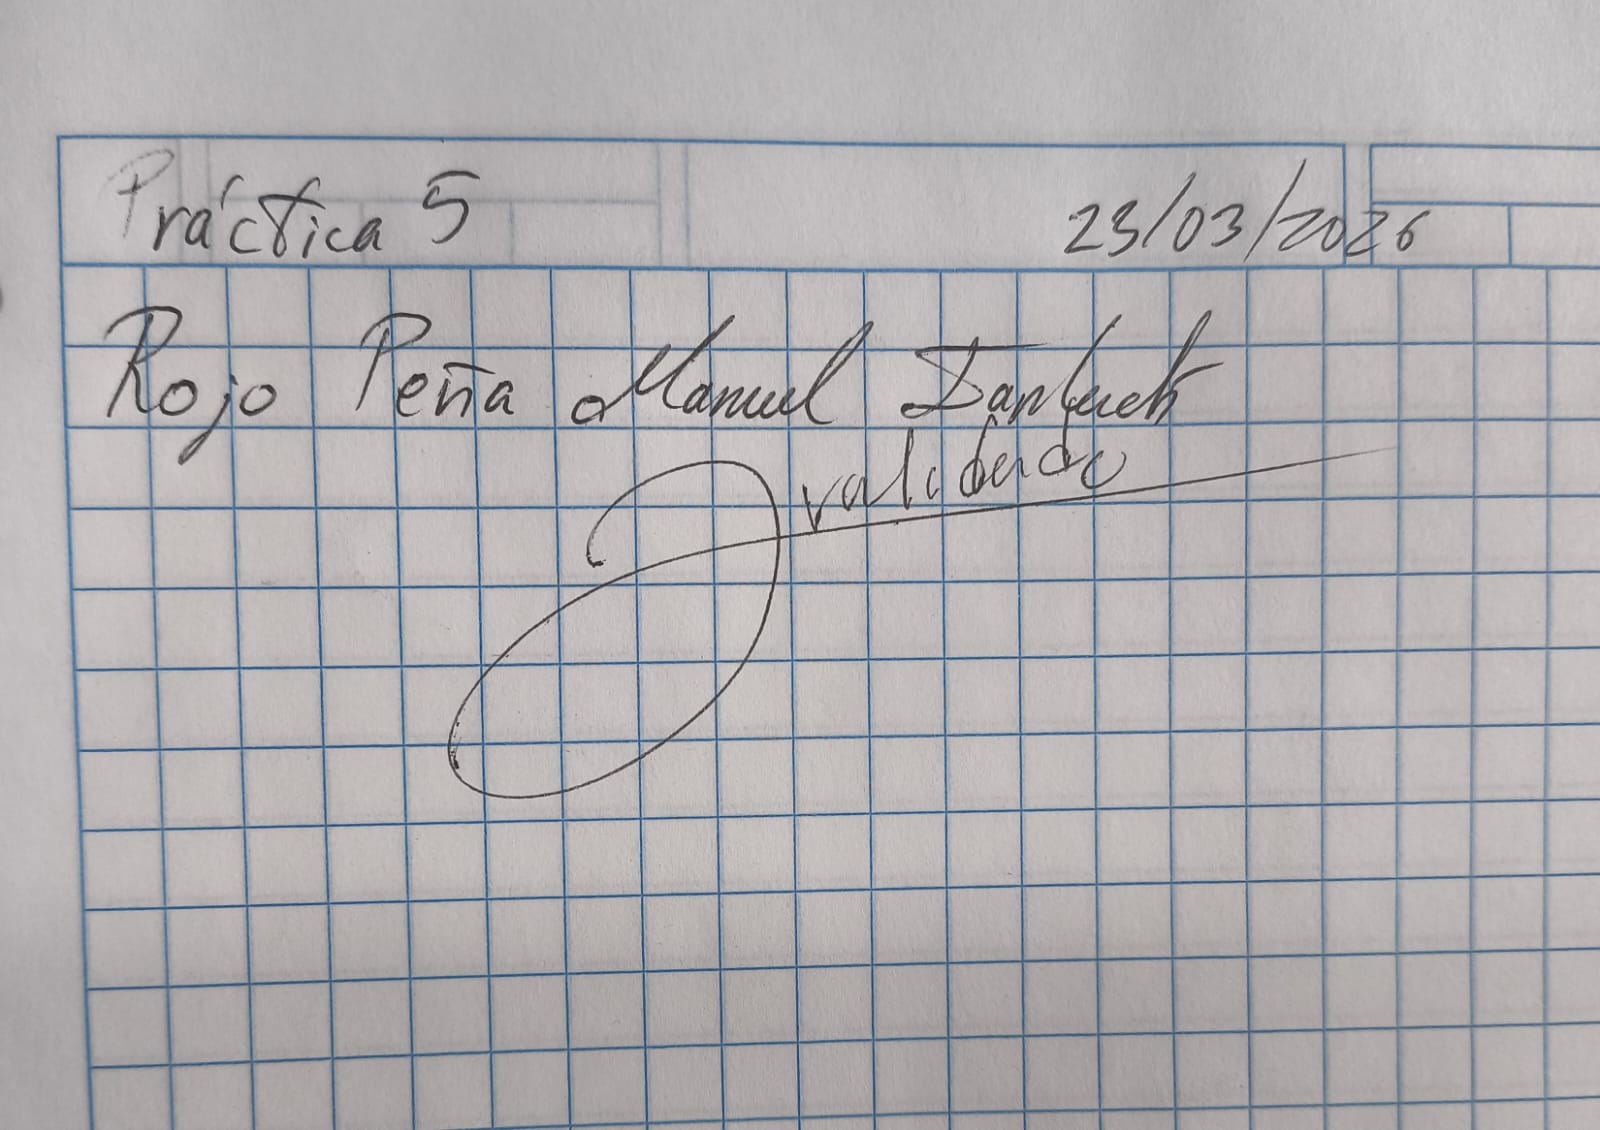
\includegraphics[width=\textwidth,height=0.97\textheight,keepaspectratio]{val.jpg}
\end{center}
 
\newpage

\section*{Conclusiones}
En la \textbf{Fase A} comprobamos que un planificador \textit{Round Robin} puro, sin ninguna primitiva de sincronización, no garantiza la integridad de los recursos compartidos. El fallo del \texttt{UART} no fue visible de forma espectacular porque la pila \texttt{USB-CDC} del \texttt{RP2040} actúa como un buffer intermediario que absorbe colisiones de escritura a pequeña escala; no obstante, al incrementar la carga se produjo el colapso de la terminal, evidenciando que la condición de carrera existe aunque no siempre sea perceptible a simple vista.\\

En la \textbf{Fase B} demostramos que dos semáforos bien diseñados son suficientes para resolver ambas condiciones de carrera de forma simultánea. El semáforo contador \texttt{sem\_energia} (init\,=\,3) mantuvo invariablemente el límite de tres calentadores activos, y el mutex \texttt{sem\_radio} (init\,=\,1) garantizó mensajes \texttt{UART} secuenciales y legibles. El truncamiento observado en la terminal es una limitación de la capa de transporte USB y no de la lógica de sincronización, lo que confirma que el kernel funciona correctamente.\\

\noindent
Desde el punto de vista del diseño, el aspecto más relevante es la \textbf{ausencia de busy-waiting}: al bloquearse, una tarea cambia su estado a \texttt{BLOCKED} y cede el CPU mediante \texttt{PendSV}, consumiendo exactamente cero ciclos hasta ser reactivada por \texttt{sem\_post}. Esto no solo es correcto, sino eficiente, pues el procesador puede atender otras tareas o entrar en modo de bajo consumo (\texttt{WFI}) durante el tiempo de espera.\\

Finalmente, al implementar esta práctica, ilustramos un principio fundamental del diseño de sistemas embebidos en tiempo real, el cual es que, compartir recursos en un entorno concurrente siempre requiere sincronización explícita. La ilusión de que el sistema ``\textit{funciona}'' sin ella es precisamente la condición más peligrosa, pues los fallos se manifiestan de forma intermitente y difícil de reproducir, exactamente como se observó en el \textit{Caso 1} de la \textbf{Fase A}.
 
\end{document}
